\subsection{Language Agnostic Features}\label{agfeatures}
This chapter details the language agnostic features that were implemented during the project. The implementation was heavily guided by the language server protocol and state of the art IDE integrations of well established languages. With these features the main goal was determining what programmers have become accustomed to when using an IDE and which features bring the biggest improvements regarding productivity. To get programmers to look deeper into the features that Dafny offers, it is important common tasks like navigating in a code base just work, because otherwise interest to learn new things fades quickly. \newline
The details of the implementation can be found in the appendix \ref{features} or in the API documentation when even more detail is desired. This chapter simply aims to explain why certain features were chosen and what improvements they bring to the daily routine of a programmer \newline

\subsubsection{CodeLenses} \label{agcodelenses}

\paragraph{What are Code Lenses}
CodeLenses in Visual Studio Code are a feature which is also common to many other IDEs. The idea is to display meta information about certain pieces of codes, for instance classes and methods. In Visual Studio Code this is done  by adding an additional line of text to the editor wherever a codeLense should  be placed. \newline
\begin{figure}[H]
	\centering
	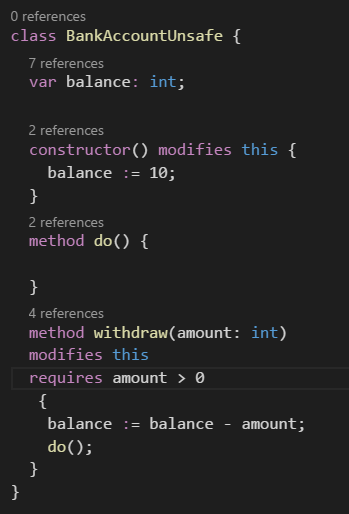
\includegraphics[width=0.5\textwidth]{img/codelensesClosed}
	\caption{Code Lenses used with Dafny}
	\label{fig:agcodelensesclosed}
\end{figure}

When given locations of the references, it is possible to let Visual Studio Code highlight them in the preview window which opens when a codeLens is expanded. Visual Studio Code also groups references according to the file path in the location, so the programmer gets to see a map of all references ordered by containing file to the right of the preview window and can quickly navigate to them.

\paragraph{Why were they chosen to implement}
Since codeLenses can be used to quickly gain a deeper understanding of a code base, it was decided to integrate this feature. Another reason was that it is widespread in different IDEs, so that programmers have become accosted to it. \newline

The first decision to be made was for which elements in the code codeLenses should be displayed. The trade off here is to  provide enough information to work comfortably with the code base and not to clutter the workspace with codeLenses It was decided to display codeLenses for classes, methods (including constructors) and fields, since they tend to have a wide scope in the code bases \newline

A second consideration was which information should be displayed in a codeLens. When codeLenses are language specific and do not for instance stem from a plugin which displays code metrics or similar, usually references and usages of the element are displayed. Since this allows the programmer to gain a deeper understanding of control flow and regions affected by refactoring, it was decided to display this information also for the Dafny plugin. CodeLenses also allow commands to be executed when clicked upon, a logical conclusion is to implement go to reference when a reference in a codeLens is clicked.\newline

\begin{figure}[H]
	\centering
	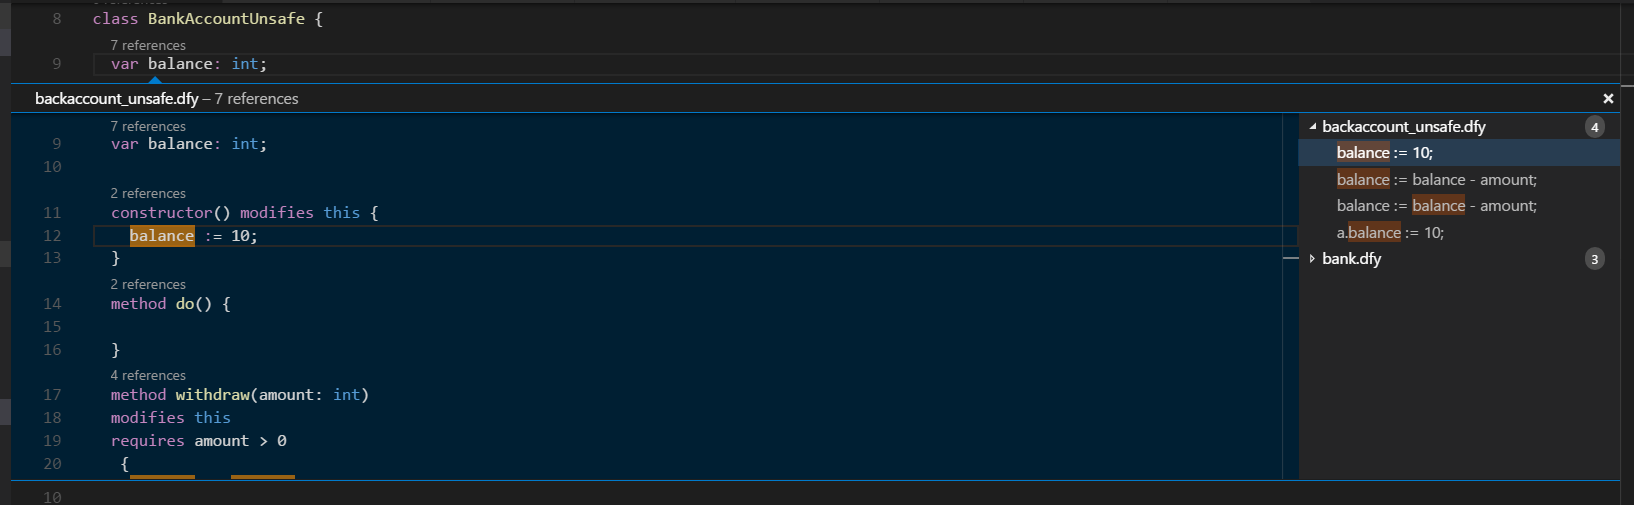
\includegraphics[width=1\textwidth]{img/codelensesExpanded}
	\caption{Expanded codeLens showing the references to the field balance}
	\label{fig:agcodelensesexpanded}
\end{figure}


\paragraph{What benefits do they entail}
CodeLenses allow to gain understanding of a code base rapidly. Scoping is visible at a glance, making it excellent to find out which regions of code are affected by a refactoring or how many classes rely on another class. By clicking on the references that are listed, one can also navigate the code base with ease, making it easy to follow program flow. \newline
The existing solutions do not yet implement code lenses at all, a feature which is wide spread in other established language integrations. Once a programmer is used to working with code lenses, it usually becomes a feature that is quite heavily used and bring a big improvement in productivity, since relationships do not have to be recorded in a mental model. It stands to reason that this feature brings the biggest improvement in understanding control flow and navigating a code base when compared to other stand alone features, making it an  important part of the plugin. \newline


\subsubsection{Code Completion} \label{agcodecompletion}

\paragraph{What is Code Completion}
Code completion prevents the programmer having to type out every identifier fully. Microsoft calls this feature IntelliSense in its products. Usually, when the programmer starts typing, a little popup appears in which the programmer can choose options that complete the code he is currently writing. The suggestions are usually context aware, because a popup that is cluttered with every identifier in the file currently opened does not bring an improvement in productivity.\newline
\begin{figure}[H]
	\centering
	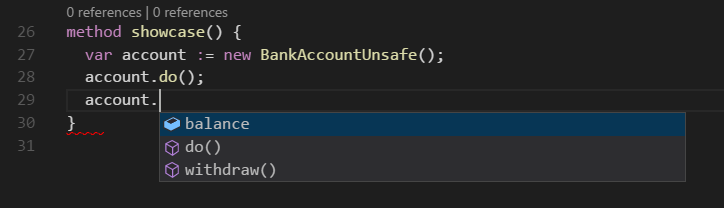
\includegraphics[width=1\textwidth]{img/codeCompletionOverview}
	\caption{Popup with completion options}
	\label{fig:agcodecompletionoverview}
\end{figure}

\paragraph{Why was it chosen to implement}
Since this is arguably one of the most helpful features in IDEs, the implementation thereof was paramount to the completion of this project. Programming in most environments, after the desired algorithm has been thought of, has become equal to the task of writing a few letters and then looking at the completion suggestions of the IDE.  \newline
Almost all modern IDEs offer a way to trigger code completion and this feature is heavily used. The main reason it was chosen to implement is that it brings very big improvements in productivity, freeing the programmer from having to remember all identifiers correctly and having to type them completely.

\paragraph{What benefits does it entail}
As already detailed, the improvement in productivity is huge when using this feature. A programmer that is used to code completion probably never wants to switch back to not using it. Amongst the existing solutions, only the Visual Studio integration offer code completion. This project however tried to go a little further and next to visually distinguishing the types of suggestions (e.g. methods, fields and so on), it also displays existing preconditions of methods in the suggestion popup. \newline

\begin{figure}[H]
	\centering
	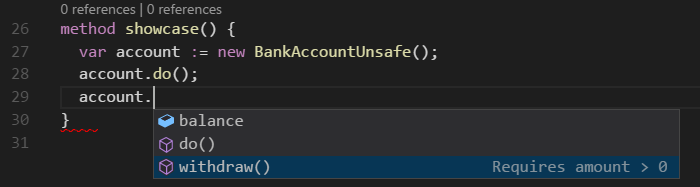
\includegraphics[width=1\textwidth]{img/codeCompletionMethod}
	\caption{Suggestion displaying precondition}
	\label{fig:agcodecompletionmethod}
\end{figure}

This combines a Dafny specific feature with a language agnostic one and lets the programmer know as early as possible under what restrictions he is working under. Being able to provide code completion in this plugin provides programmers with the opportunity translating their thoughts quickly into code and not having to bother with exact writing. \newline

\subsubsection{Go to Definition} \label{aggotodefinition}
\paragraph{What is Go to Definition}
Another common feature in modern IDEs is go to definition. It enables the programmer to quickly jump to the definition of a code element he is currently working with in order to gain further insight about it. This can usually be done either via a hot key for the current cursor position or an option when opening the context menu via a right click, Visual Studio Code offers both ways.\newline

\begin{figure}[H]
	\centering
	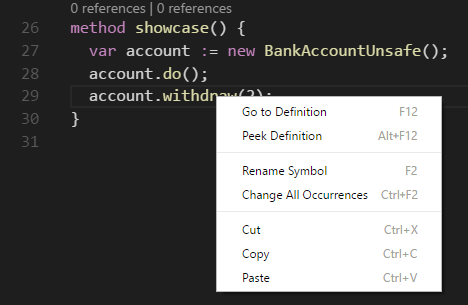
\includegraphics[width=0.5\textwidth]{img/goToDefinition}
	\caption{The Definition Features}
	\label{fig:aggotodefinition}
\end{figure}

Usually this feature offers to either open the code file containing the definition or just to peek at it in a popup. Visual Studio Code supports both these options. If the definition is ambiguous, which often happens when working with interfaces, usually a list of all possible definitions is displayed, because the concrete definition is often impossible to find using static code analysis.

\paragraph{Why was it chosen to implement}
Since, similar to codeLenses, this is a feature which is elemental to all modern IDEs and provides great overview over a project, the implementation of this feature had a high priority in this project. It is also used to navigate in a code base and is actually the reverse application of references in a codeLens, because instead of finding all usages, one jumps from a usage to the definition. \newline

Next to code completion, it is probably the feature most widely implemented in IDEs, so it is important that a Dafny integration does implement it as well, as it provides programmers an idiomatic way of working with a code base.

\paragraph{What benefits does it entail}
Similar to codeLenses, go to definition is a command which can deepen the understanding of a code base profoundly. It is at all times clear where a certain symbol comes from, and one can easily check what it does by jumping to the implementation. It also helps a lot when one has to trace control flow backwards in order to find out where certain data originates from. \newline
The existing solutions do not yet implement go to definition, with the exception of the Visual Studio integration. Being able to quickly navigate to a symbols definition keeps the programmer of having to keep track of all implementations and staying in the current scope of abstraction. If one needs to know more about a symbol, a peek can quickly show the desired information without distracting the train of thought with a new open file in the editor. This makes programmers that use this command usually more efficient and productive.\newline

\begin{figure}[H]
	\centering
	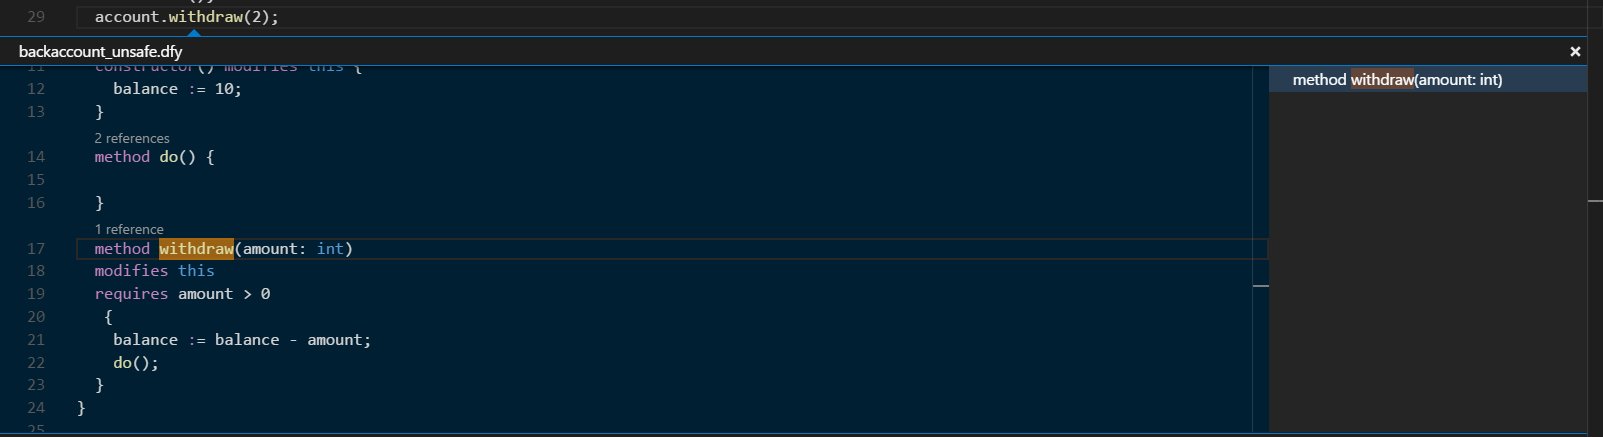
\includegraphics[width=1\textwidth]{img/goToDefinitionPeek}
	\caption{Overlay of peeked definition}
	\label{fig:aggotodefinitionpeek}
\end{figure}


\subsubsection{Rename Element} \label{agrenameelement}
\paragraph{What is Rename Element}
Rename element is a feature essential to refactoring. It is very widespread in IDEs. Visual Studio Code offers built in support for renaming either via a hot key or the context menu. Renaming an element switches all occurrences of an identifier to a new one. This can be a methods, an alias of an object or any other element in a code base. \newline

\begin{figure}[H]
	\centering
	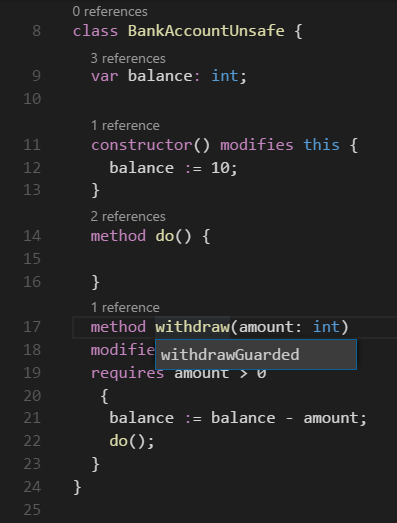
\includegraphics[width=0.5\textwidth]{img/rename}
	\caption{Renaming an element in Visual Studio Code}
	\label{fig:agrename}
\end{figure}

With this feature, one has to be careful when implementing it, since it actually changes the code base and it has to be sure which elements have to be renamed and which do not. There can be several identifiers that are exactly the same but reside in different scopes. When applying the refactoring, only the correct occurrences, which are determined by scope, should be changed while the others must stay untouched. Doing otherwise can change the expressed intent of a program or, if done poorly, can break code.

\paragraph{Why was it chosen to implement}
Because of its importance in refactoring, which is one of the most important tasks when programming, implementing this feature belongs to the core scope of this project. Renaming element allows to quickly make code better readable.\newline
Keeping a code base readable and clean should be one of the biggest concerns when developing a product, a feat which is only accomplished through constant refactoring, a task which is almost impossible to do when renaming of elements is not supported automatically should the code base grow sufficient big enough.

\paragraph{What benefits does it entail}
Renaming of elements allows the programmer to keep the expressed intent of a program in sync with the actual intent when implementations change as they tend to do over time. Normally more time in programming is spent editing or deleting old lines of code than writing new ones. Having automated support in this area does not only make work quicker, but also guarantees for non breaking changes when implemented correctly. When one has to adapt many pieces of code manually, it is almost guaranteed to make a mistake somewhere. \newline
None of the existing solutions support context aware renaming, which is very important if the refactoring should be applied correctly. When writing production quality software, renaming of elements helps to keep the intent clear and make the code base more readable, which is especially important if it has to be maintained for a long lifespan. For these reasons, a programmers that uses this feature often and correctly tends to write more expressive code.

\subsubsection{Syntax Highlighting} \label{agsyntaxhighlighting}
\paragraph{What is Syntax Highlighting}
Syntax highlighting is the feature of displaying different elements in the editor with different colors. Usually there is an IDE idiomatic coloring scheme, so that for instance all language keywords or types are colored the same across different languages, if the IDE supports multiple. \newline
\begin{figure}[H]
	\centering
	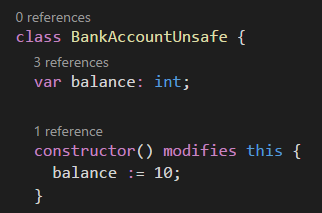
\includegraphics[width=0.5\textwidth]{img/syntaxHighlighting}
	\caption{Syntax Highlighting of Dafny}
	\label{fig:agsyntaxHighlighting}
\end{figure}
Syntax highlighting is usually applied constantly and updates instantly when the programmer types new code. The mechanisms to display the coloring are also very deeply ingrained into the IDE, relaying on a declarative language grammar definition file to do all the coloring. 

\paragraph{Why was it chosen to implement}
Syntax highlighting is definitely the first feature to get working in an IDE, maybe next to run programming. Even simple text editors such as Notepad support syntax highlighting for multiple languages, so it is expected of a language integration to come with working highlighting. \newline

\paragraph{What benefits does it entail}
This feature makes code a lot more readable, and a lot more time is spent reading code than writing. It makes the purpose of a symbol clear at first glance thanks to idiomatic coloring. Understanding code becomes much easier when one is guided by colors. Syntax highlighting can also help tracing bugs were the programmer and the compiler do not have the same opinion of a certain semantic, since syntax highlighting reflects the way a compiler interprets a piece of code. \newline
Since this is such a basic feature, all existing solution support this feature, usually relying on the same grammar definition file written for the sublime integration of Dafny \cite{sublime}. This project expanded the implementation a little, also providing syntax highlighting for parameters and generic arguments, something that existing solutions neglect.
\begin{figure}[H]
	\centering
	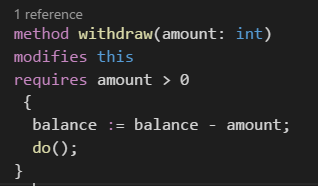
\includegraphics[width=0.5\textwidth]{img/syntaxHighlightingMethod}
	\caption{Syntax Highlighting of parameters}
	\label{fig:agsyntaxHighlightingMethod}
\end{figure}